\chapter{Explainability Case Studies}
\label{ch:explainability}

This chapter tests specific mechanistic claims made in Chapter~\ref{ch:results} with targeted diagnostics, rather than relying on the aggregate metrics alone to support the mechanisms offered there.

\section{Reconstruction-Error Localization on Yahoo A3}
\label{sec:explain-yahoo}

The A3 discussion in Chapter~\ref{ch:results} attributes the Transformer Bottleneck Autoencoder's lead over the LSTM Autoencoder (AP 0.663 vs.\ 0.392, ROC-AUC 0.813 vs.\ 0.566) to a mechanistic difference between the two bottlenecks: the LSTM Autoencoder compresses an entire 64-step window into a single final hidden state, which is hypothesized to destroy the window's seasonal phase information and produce reconstruction error that is smeared diffusely across all timesteps; the Transformer's global self-attention, by contrast, is hypothesized to preserve enough positional information to localize its reconstruction error sharply at the specific timestep where the window's phase is violated. This is a plausible mechanism, but as stated it is inferred from the aggregate metrics alone -- neither model's per-timestep error was actually inspected. This section tests it directly.

\subsection{Initial Assumption}

The hypothesis under test makes an explicit, checkable prediction: for anomalous A3 windows, the LSTM Autoencoder's per-timestep squared reconstruction error should look approximately \emph{uniform} across the window's 64 positions, while the Transformer's per-timestep error should show a sharp, localized peak at the position where the seasonal pattern is violated. If instead both models produce similarly shaped error profiles, the AP/ROC-AUC gap would need a different explanation than the one offered.

\subsection{Qualitative Check: Per-Timestep Error Heatmaps}

Both trained models were reconstructed on every anomalous A3 test window, and the per-timestep squared error was plotted as a heatmap (one row per window, one column per of the 64 timesteps), with a random subsample of 300 windows used to keep the rendered image legible. Figures~\ref{fig:explain-lstm-heatmap} and~\ref{fig:explain-transformer-heatmap} show the result.

\begin{figure}[H]
\centering
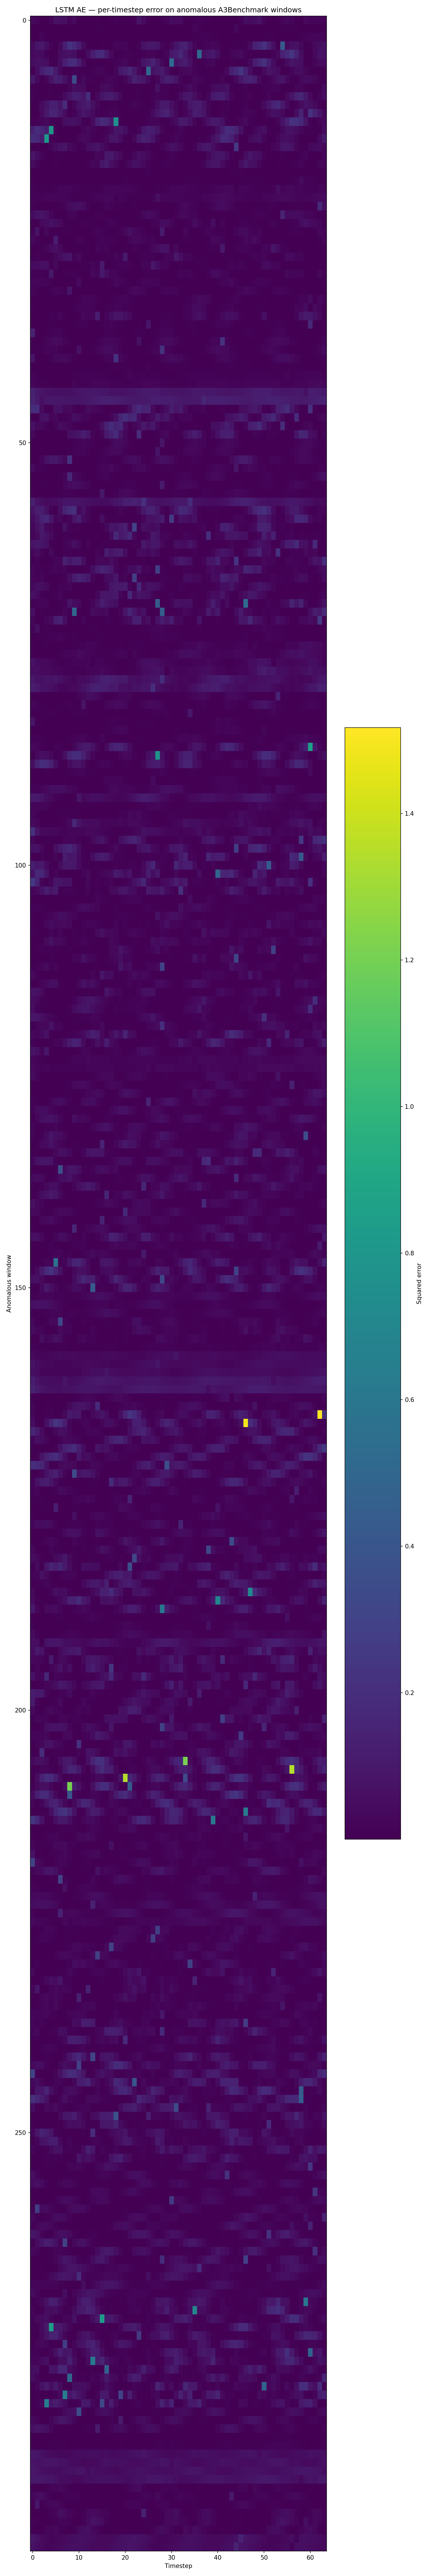
\includegraphics[height=0.55\textheight,keepaspectratio]{../../data/explainability/yahoo_A3Benchmark_lstm_vs_transformer/5/lstm_ae_error_heatmap.png}%
\hspace{0.04\textwidth}%
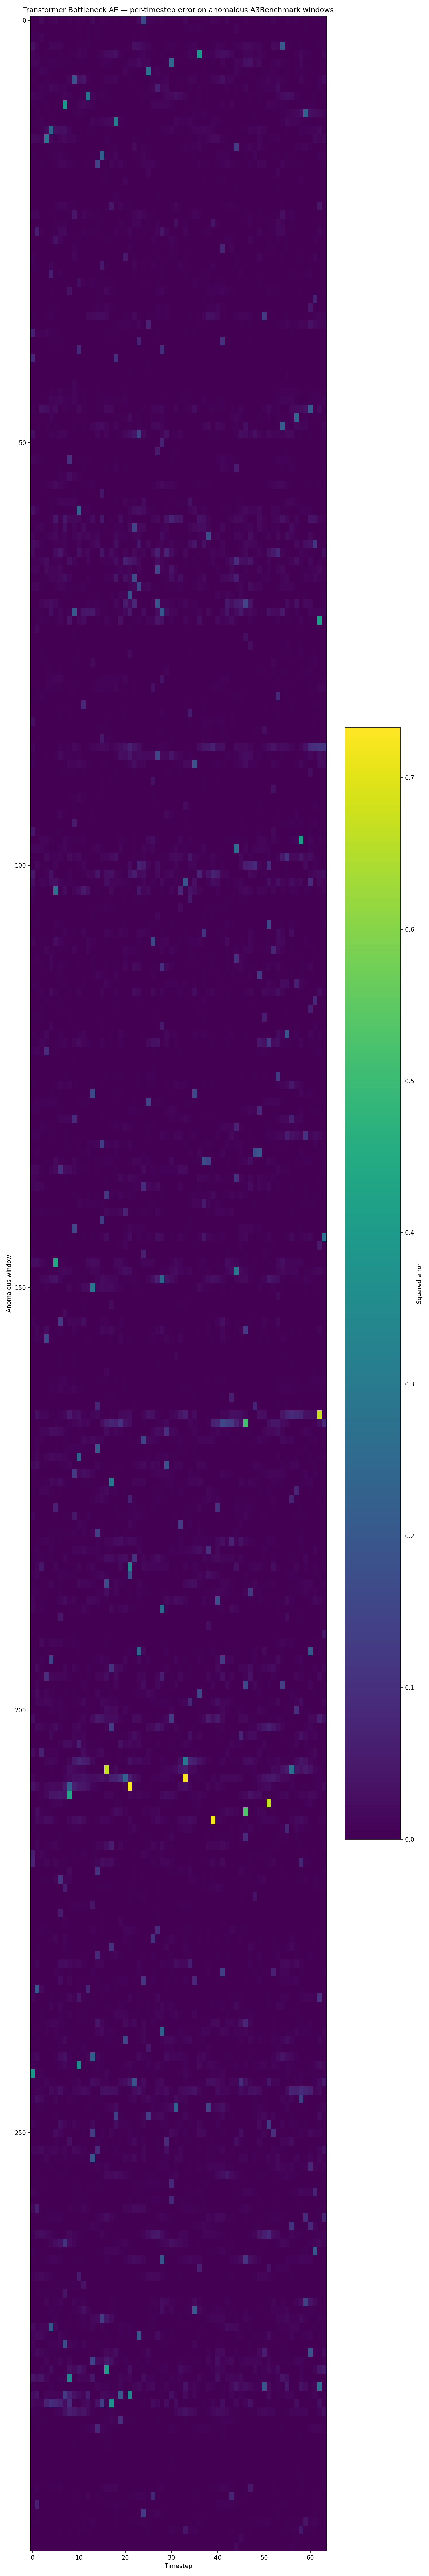
\includegraphics[height=0.55\textheight,keepaspectratio]{../../data/explainability/yahoo_A3Benchmark_lstm_vs_transformer/5/transformer_bottleneck_error_heatmap.png}

\caption{LSTM Autoencoder -- per-timestep squared reconstruction error on 300 randomly sampled anomalous A3 windows (one row per window, left). Elevated error appears as sparse, punctate points rather than as a uniform band, but a visibly larger share of rows carry a low-level elevated baseline across most of their width compared to the Transformer.}
\label{fig:explain-lstm-heatmap}
\caption{Transformer Bottleneck Autoencoder -- per-timestep squared reconstruction error on the same 300 anomalous A3 windows, same row order and colour scale convention as Figure~\ref{fig:explain-lstm-heatmap} (right). Error is visibly more sparse and confined to isolated timesteps.}
\label{fig:explain-transformer-heatmap}
\end{figure}

The visual comparison is broadly consistent with the initial assumption -- the Transformer's error concentrates into fewer, brighter points, while the LSTM Autoencoder's error is more often spread thinly across a window's full width -- but a heatmap read by eye is a weak instrument here: each panel is normalized to its own colour scale, and the LSTM Autoencoder's error values are roughly double the Transformer's in magnitude throughout, which alone would make its background look more saturated regardless of how concentrated the error actually is. A qualitative read of Figures~\ref{fig:explain-lstm-heatmap}--\ref{fig:explain-transformer-heatmap} therefore \emph{suggests} the phase-destruction mechanism but cannot confirm it.

\subsection{Quantitative Verification: Gini Coefficient of Error Concentration}

To separate genuine error concentration from an artifact of differing overall error magnitude, each anomalous window's 64 per-timestep squared errors were summarized with a Gini coefficient -- a standard inequality measure (originally used for income distributions) that is invariant to the absolute scale of its input. For a window's 64 error values sorted ascending, a Gini of 0 means the error is spread perfectly evenly across every timestep, and a Gini of 1 means it is concentrated entirely at a single timestep; unlike a raw magnitude comparison, this metric isolates the \emph{shape} of the error distribution within a window from its overall size.

For $n$ per-timestep squared errors $x_1 \le x_2 \le \dots \le x_n$ sorted ascending (here $n=64$), the Gini coefficient is computed as

\begin{equation}
G = \frac{2 \sum_{i=1}^{n} i \, x_i}{n \sum_{i=1}^{n} x_i} - \frac{n+1}{n}.
\label{eq:gini}
\end{equation}

Computed over the full population of 14{,}449 anomalous A3 windows, the two models separate clearly:

\begin{center}
\begin{tabular}{@{}lll@{}}
\toprule
 & Mean Gini & Median Gini \\
\midrule
LSTM Autoencoder & 0.566 & 0.606 \\
Transformer Bottleneck Autoencoder & 0.721 & 0.724 \\
\bottomrule
\end{tabular}
\end{center}

\begin{figure}[H]
\centering
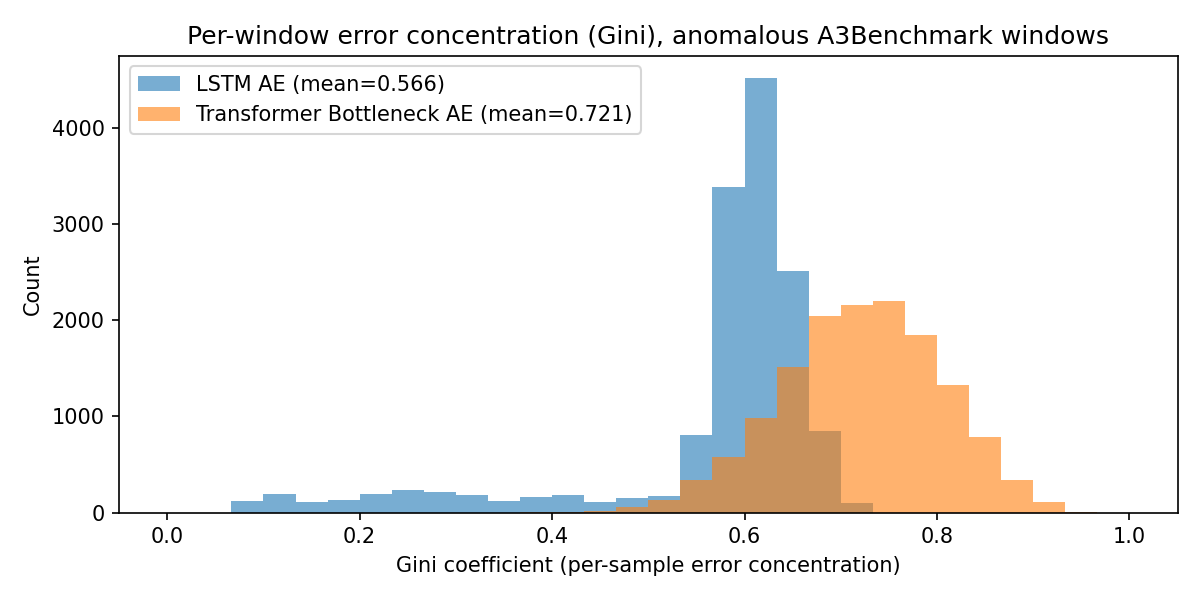
\includegraphics[width=0.7\textwidth]{../../data/explainability/yahoo_A3Benchmark_lstm_vs_transformer/5/gini_comparison.png}
\caption{Distribution of per-window Gini coefficients across all 14{,}449 anomalous A3 windows. The Transformer's distribution is unimodal and shifted toward high concentration (Gini $>0.6$); the LSTM Autoencoder's distribution is bimodal, with a majority clustered near the Transformer's range but a distinct secondary population spread across low Gini values (error genuinely smeared across the window).}
\label{fig:explain-gini}
\end{figure}

This confirms the initial assumption on average: the Transformer's error is more concentrated than the LSTM Autoencoder's across the full anomalous population, not merely in the handful of examples a heatmap happens to display. But the distribution in Figure~\ref{fig:explain-gini} reveals a detail the aggregate means alone would miss -- the LSTM Autoencoder's Gini values are \emph{bimodal}, not uniformly shifted down. A majority of its windows cluster in essentially the same high-concentration range as the Transformer's (Gini $\approx 0.6$, comparable localization ability), while a distinct secondary population of windows sits at low Gini ($<0.4$), where the error genuinely is smeared close to evenly across the full window. This indicates the phase-destruction mechanism is not a uniform property of every LSTM Autoencoder reconstruction, but a failure mode affecting a specific subset of windows -- and it is this subpopulation, not a general degradation across all anomalous windows, that is responsible for dragging the LSTM Autoencoder's aggregate AP and ROC-AUC below the Transformer's, since on the remaining majority of windows the two models localize error comparably well.

\section{Pseudo-Sequence Reconstruction Error on Credit Card Fraud}
\label{sec:explain-cc}

The Credit Card Discussion in Chapter~\ref{ch:results} argues that the three "temporal" architectures (Predictive LSTM, LSTM Autoencoder, Transformer Bottleneck Autoencoder) do not see a genuine sequence: each reshapes a row's 29 independent, decorrelated PCA features into an artificial sequence of 29 scalar steps, in whatever order the columns happen to appear in the source CSV. Predictive LSTM's poor performance (AP 0.519) is attributed directly to this -- "adjacent PCA components are orthogonal/decorrelated by construction, so there is no real next-step signal to learn." This section tests the reconstruction-based half of that claim (LSTM Autoencoder, Transformer Bottleneck Autoencoder) with the same per-position error diagnostic used in \S\ref{sec:explain-yahoo}.

\subsection{Initial Assumption}

If the 29 column positions genuinely carry no meaningful order, per-position reconstruction error on fraud samples should look like unstructured noise: no column should consistently accumulate more error than any other across the fraud population, for either model. A structured, repeated pattern -- specific columns lighting up across many fraud samples -- would complicate that picture and call for a follow-up explanation.

\subsection{Qualitative Check: Per-Feature-Position Error Heatmaps}

Both trained models were reconstructed on the full fraud test population (492 samples), and the per-column squared error was plotted as a heatmap (one row per sample, one column per of the 29 feature positions), with a random subsample of 300 fraud samples used to keep the rendered image legible. Figures~\ref{fig:explain-cc-lstm-heatmap} and~\ref{fig:explain-cc-transformer-heatmap} show the result.

\begin{figure}[H]
\centering
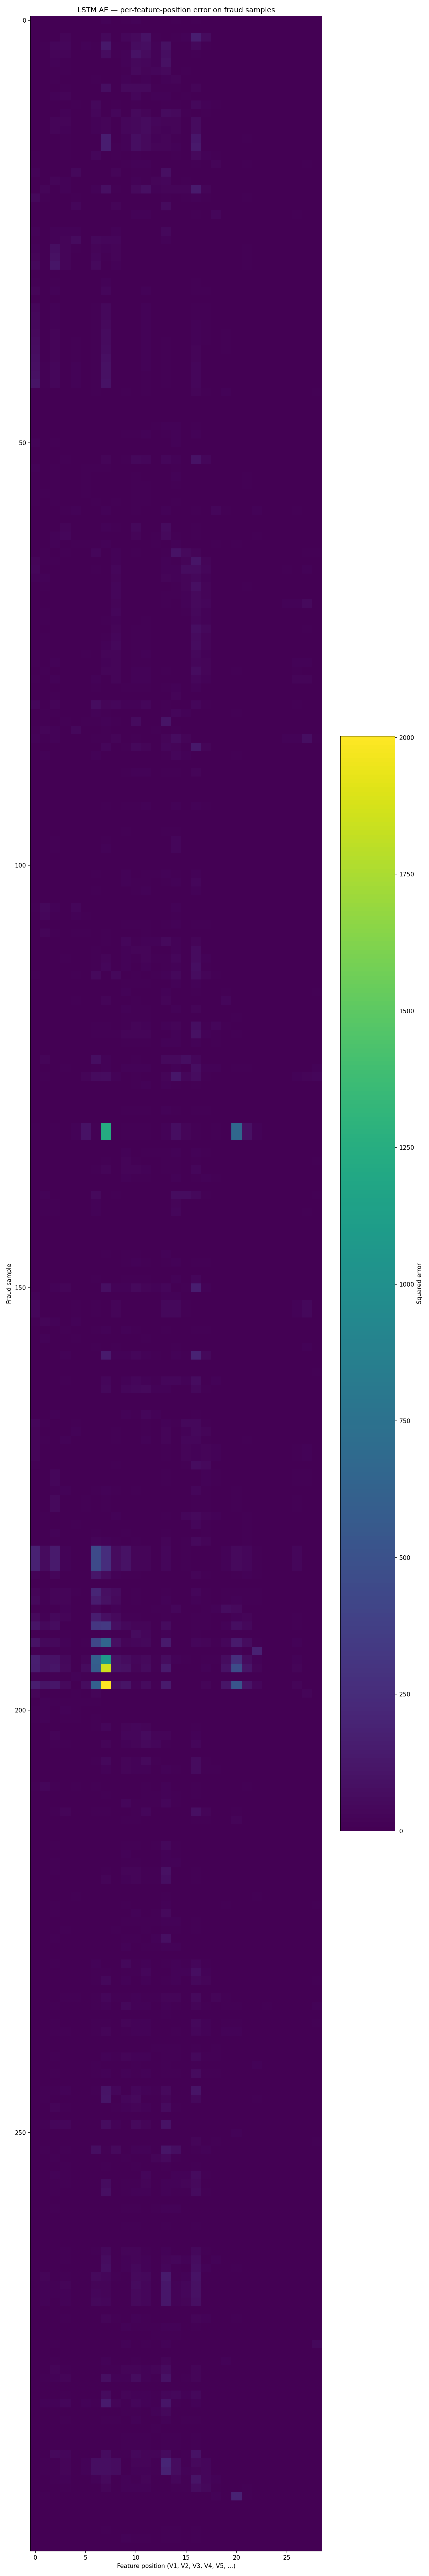
\includegraphics[height=0.55\textheight,keepaspectratio]{../../data/explainability/credit_card_lstm_vs_transformer/5/lstm_ae_error_heatmap.png}%
\hspace{0.04\textwidth}%
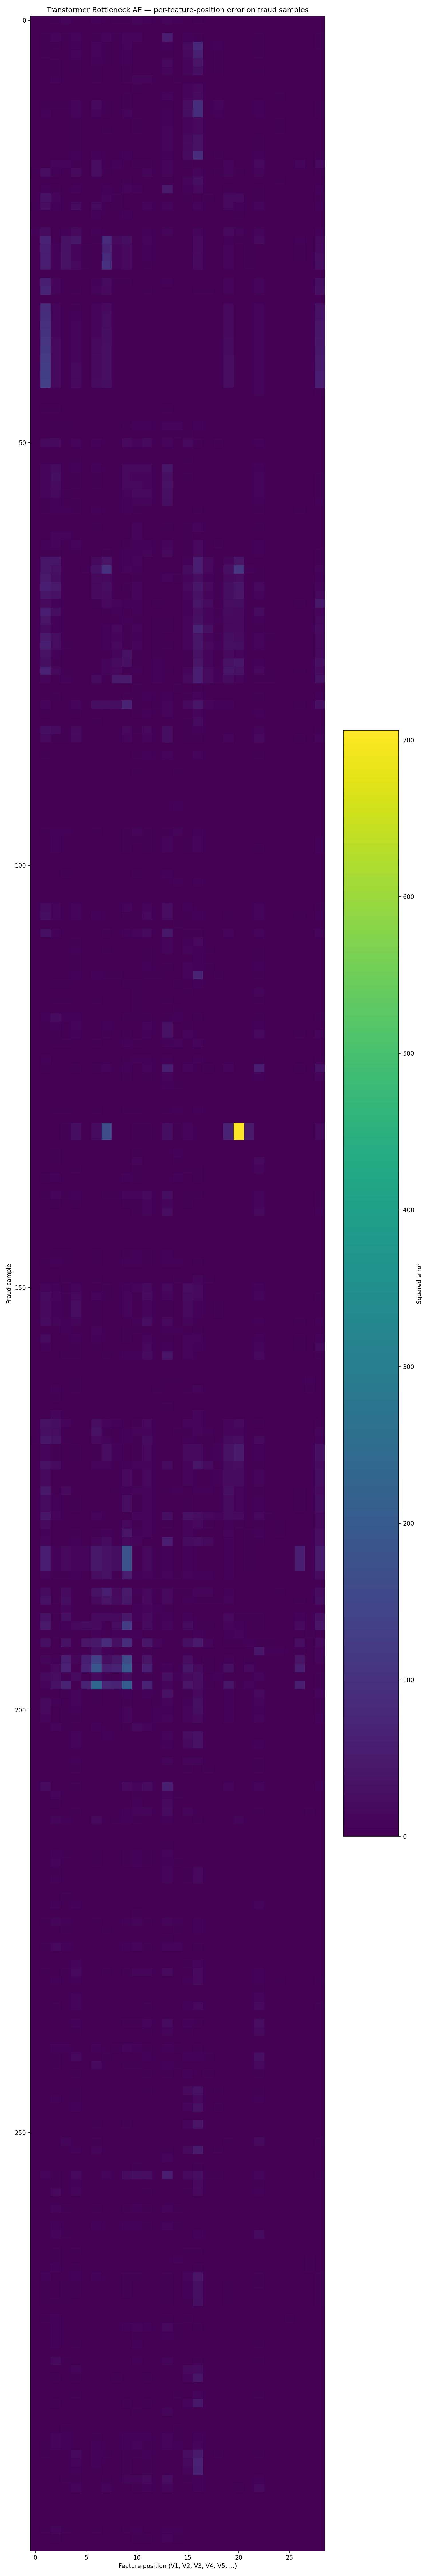
\includegraphics[height=0.55\textheight,keepaspectratio]{../../data/explainability/credit_card_lstm_vs_transformer/5/transformer_bottleneck_error_heatmap.png}

\caption{LSTM Autoencoder -- per-feature-position squared reconstruction error on 300 randomly sampled fraud transactions (one row per sample, columns V1--V28 then Amount, left).}
\label{fig:explain-cc-lstm-heatmap}
\caption{Transformer Bottleneck Autoencoder -- per-feature-position squared reconstruction error on the same 300 fraud transactions, same row order and column convention as Figure~\ref{fig:explain-cc-lstm-heatmap} (right).}
\label{fig:explain-cc-transformer-heatmap}
\end{figure}

Contrary to the initial assumption, both heatmaps show a visibly structured, repeated pattern: a handful of column positions accumulate elevated error across many fraud rows, rather than error being scattered evenly across all 29 positions. This does not by itself contradict the "no real sequence" claim -- it does not show that the models exploit \emph{order}, only that error is not uniformly distributed across \emph{columns}. Two distinct explanations are consistent with a structured heatmap: either specific PCA features are simply harder to reconstruct on fraud rows regardless of where they sit in the row (a feature-\emph{identity} effect, fully compatible with "no real sequence"), or the models are exploiting some incidental adjacency between specific neighbouring columns in this one fixed ordering (a position effect, which would nuance but not overturn the claim, since that adjacency is still arbitrary and non-causal). The heatmap alone cannot distinguish these.

\subsection{Quantitative Verification: Column-Shuffle Feature-Identity Check}

To separate the two explanations, the same 492 fraud rows were re-run through both models with a fixed random permutation of the 29 columns applied first (seed 42), and the per-column error was re-ranked. If the same underlying features dominate the top-error positions in both the original and the shuffled column order, the effect is feature-identity-driven; if overall error also changes substantially after shuffling, position/adjacency plays a role too.

\begin{center}
\resizebox{\textwidth}{!}{%
\begin{tabular}{@{}lccl@{}}
\toprule
 & Overlap (top 10, orig.\ vs.\ shuffled) & Top-error magnitude, orig.\ $\to$ shuffled & Stable top features (in both orderings) \\
\midrule
LSTM Autoencoder & 6/10 & 47.7 $\to$ 71.7 & V1, V3, V7, V8, V14, V17 \\
Transformer Bottleneck AE & 6/10 & 12.9 $\to$ 136.8 & V2, V3, V7, V8, V14, V17 \\
\bottomrule
\end{tabular}%
}
\end{center}

Both effects are present. Six of the top 10 highest-error features are the same before and after shuffling, for both models -- well above the $\sim$3--4 expected in common between two independent random top-10 draws out of 29 features under a pure-noise null. \textbf{V14 and V17 are stable top accumulators for both models under both orderings}, and both are independently singled out by the community exploratory notebook cited in Chapter~\ref{ch:methodology} as its two strongest negative correlates with the fraud label -- an external check that these two features genuinely carry fraud-relevant signal, not an artifact of this experiment. At the same time, overall error rose substantially after shuffling for both models (LSTM Autoencoder's top value: 47.7 $\to$ 71.7; Transformer's: 12.9 $\to$ 136.8), which only makes sense if both encoders were also leaning on some incidental adjacency between specific neighbouring columns in the fixed, original CSV order.

Taken together, this confirms the core claim with a refinement the aggregate metrics could not surface on their own: the reconstruction-based architectures did learn to depend on the one fixed, arbitrary column ordering supplied at preprocessing time, beyond what a pure feature-identity effect would predict. The fact that error went up means the models had implicitly learned something that depended on which value sat next to which in the specific column arrangement the CSV happens to use, even though that adjacency is meaningless (it's just PCA-component arbitrary order)
 - not evidence of a hidden causal sequence in the data, but more like the models overfit to an arbitrary but fixed layout

\section{Disjoint Feature Regimes: AE+Context vs.\ Temporal IForest}
\label{sec:explain-disjoint-regime}

The CIC-IDS2017 Discussion in Chapter~\ref{ch:results} proposes pairing AE+Context (strong on DDoS and PortScan) with Temporal IForest (strong on the slow-DoS classes and, tentatively, Heartbleed) into a practical ensemble, since the two operate on disjoint feature regimes -- host-context features versus a 16-flow temporal window. That argument rests on two separate premises, one per model: that Temporal IForest's score is genuinely informed by the window's temporal structure rather than by one flow's static feature values sitting inside a wider, functionally inert vector; and that AE+Context's score is genuinely informed by the host-context features unique to it, rather than by the same flow-level features Temporal IForest already has access to. Both are tested in turn below.

\subsection{Temporal IForest: Initial Assumption}

If Temporal IForest is genuinely exploiting cross-timestep structure, its per-window score should remain informative about the \emph{last} flow's own label -- the flow that would be paired with AE+Context's per-flow score in the ensemble -- rather than only about whether \emph{some} flow within the 16-flow window is an attack. Its SHAP attribution should also not collapse onto that single last flow; if it does, the window is decorative and the ``disjoint feature regime'' argument for the ensemble does not hold.

\subsection{Temporal IForest: Score Validity Under Last-Flow Labeling}

The originally showed per-class AP figures use an ``any-of-16'' window label: a window is positive if any of its 16 flows is an attack, tagged with the majority attack type. That is more lenient than the per-flow labeling AE+Context is scored against. Every existing test window was relabeled by its \emph{last} flow's own true label instead, and per-class AP recomputed against the unchanged, already-trained model and its existing scores.

\begin{center}
\begin{tabular}{@{}lccc@{}}
\toprule
 & AP (any-of-16) & AP (last-flow) & $n$ (last-flow) \\
\midrule
DDoS              & 0.9518 & 0.9515 & 95{,}123 \\
DoS GoldenEye     & 0.6278 & 0.6265 & 7{,}567 \\
DoS Slowhttptest  & 0.6851 & 0.6849 & 1{,}742 \\
DoS slowloris     & 0.6091 & 0.6077 & 4{,}001 \\
Heartbleed        & 0.5927 & 0.2892 & 11 \\
\bottomrule
\end{tabular}
\end{center}

We see AP is essentially unchanged for all four target classes under the stricter labeling, confirming the score is informative about the last flow's own status, not an artifact of the lenient window label. Heartbleed drops sharply, but on only 11 true flows -- its entire test population -- so it is excluded from the ensemble and treated as tentative, consistent with its hedged treatment in Chapter~\ref{ch:results}.

\subsection{Temporal IForest: SHAP Attribution Across the Window}
\label{sec:explain-temporal-window}

Temporal IForest is trained on flattened 16-flow windows, so \texttt{TreeExplainer}'s SHAP values on the flattened input decompose cleanly back into a (window, timestep, feature) cube. For each of the four classes, SHAP was computed on 200 windows; attribution magnitude was summed over features per timestep to check for concentration on the final timestep, and the top contributing features were plotted across all 16 timesteps to check whether the same feature carries consistent-sign attribution throughout the window rather than only near the end.

\begin{figure}[H]
\centering
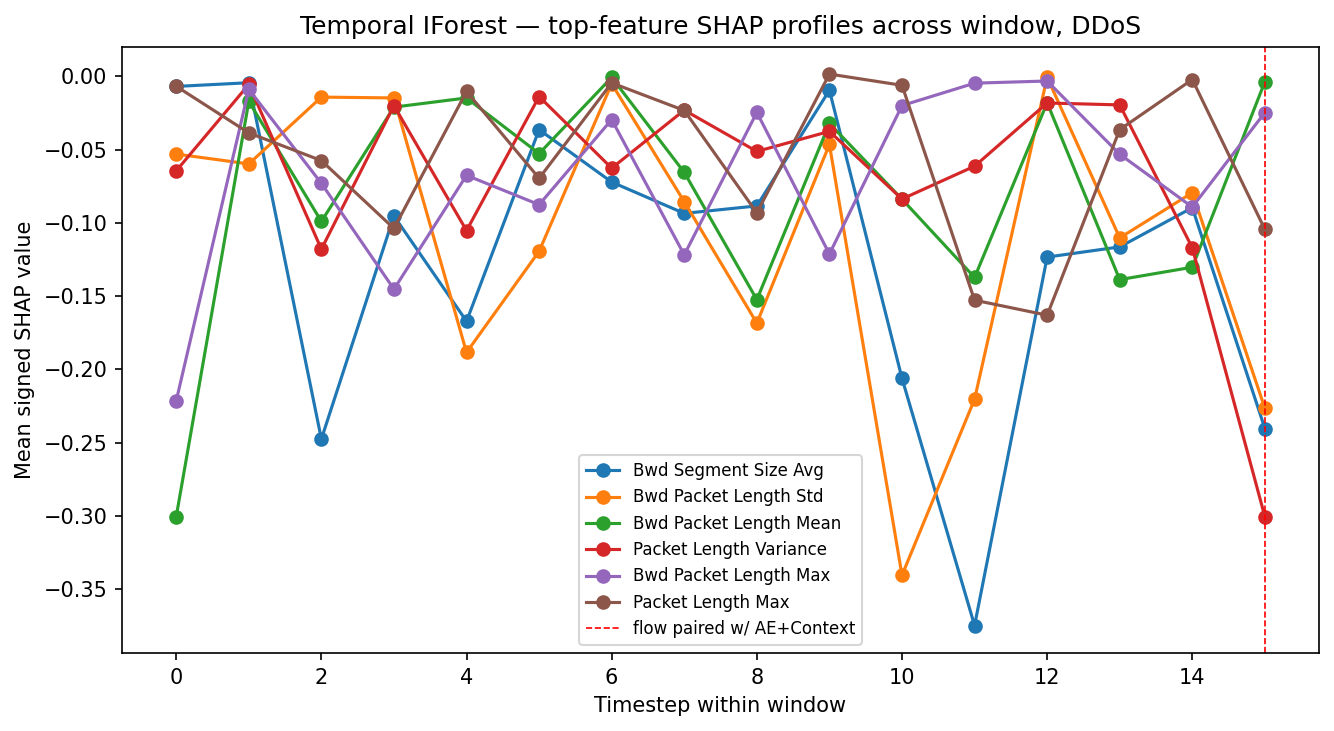
\includegraphics[width=0.48\textwidth,keepaspectratio]{../../data/explainability/cicids_temporal_shap/1/ddos_top_feature_profiles.png}%
\hspace{0.02\textwidth}%
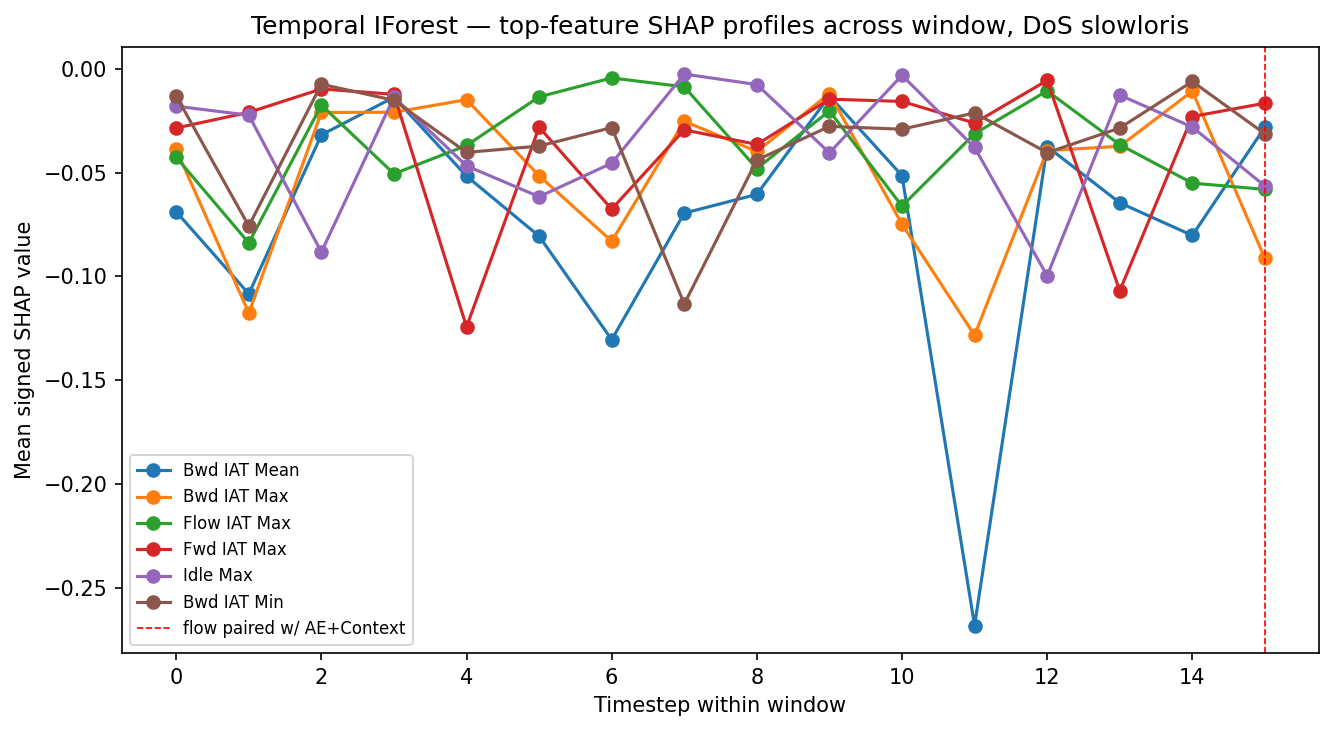
\includegraphics[width=0.48\textwidth,keepaspectratio]{../../data/explainability/cicids_temporal_shap/1/dos_slowloris_top_feature_profiles.png}

\caption{Temporal IForest -- mean SHAP value per timestep for the six most-attributed features, DDoS windows (left) and DoS slowloris windows (right). In both cases attribution is negative (anomalous), recurs at consistent sign across most of the 16 timesteps, and does not concentrate at the final flow (dashed red line) -- the flow paired with AE+Context's score in the proposed ensemble.}
\label{fig:explain-temporal-shap}
\end{figure}

\begin{figure}[H]
\centering
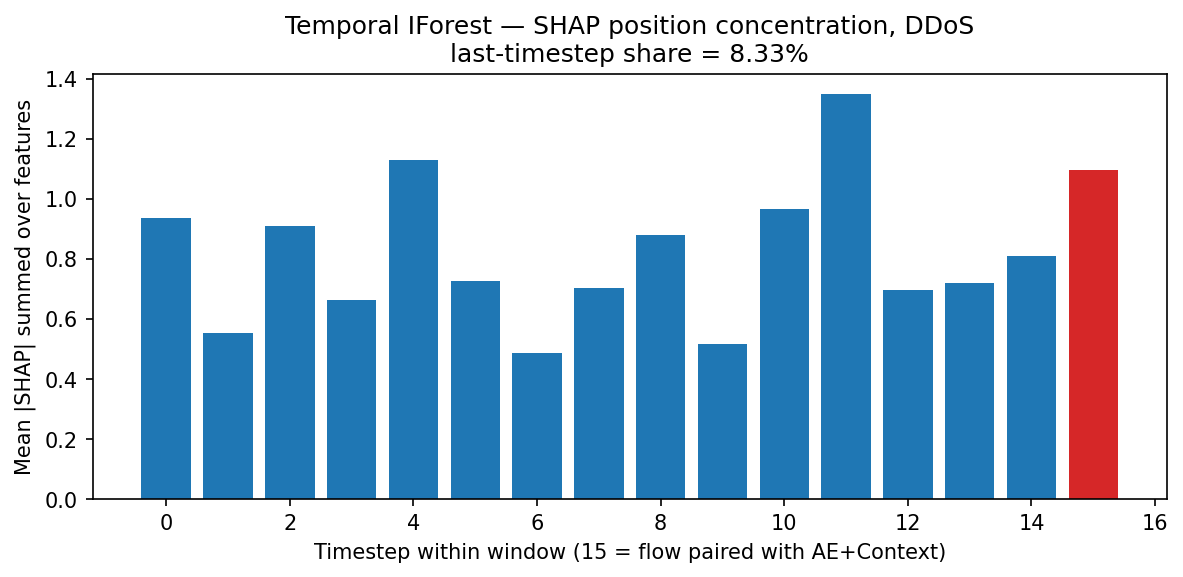
\includegraphics[width=0.48\textwidth,keepaspectratio]{../../data/explainability/cicids_temporal_shap/2/ddos_position_concentration.png}%
\hspace{0.02\textwidth}%
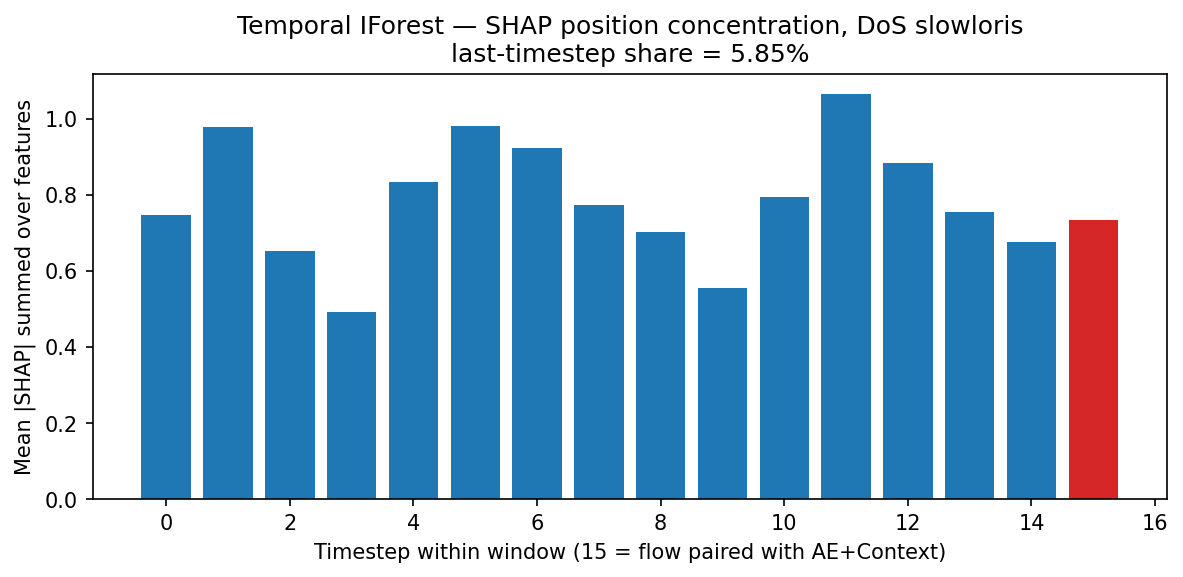
\includegraphics[width=0.48\textwidth,keepaspectratio]{../../data/explainability/cicids_temporal_shap/2/dos_slowloris_position_concentration.png}
\caption{Temporal IForest -- mean $|\text{SHAP}|$ summed over features, per timestep, DDoS windows (left) and DoS slowloris windows (right). The final timestep (red bar, 15) -- the flow paired with AE+Context's score in the proposed ensemble -- carries no more attribution mass than any other position in the window, confirming the summary statistic reported below.}
\label{fig:explain-temporal-position-concentration}
\end{figure}

\begin{figure}[H]
\centering
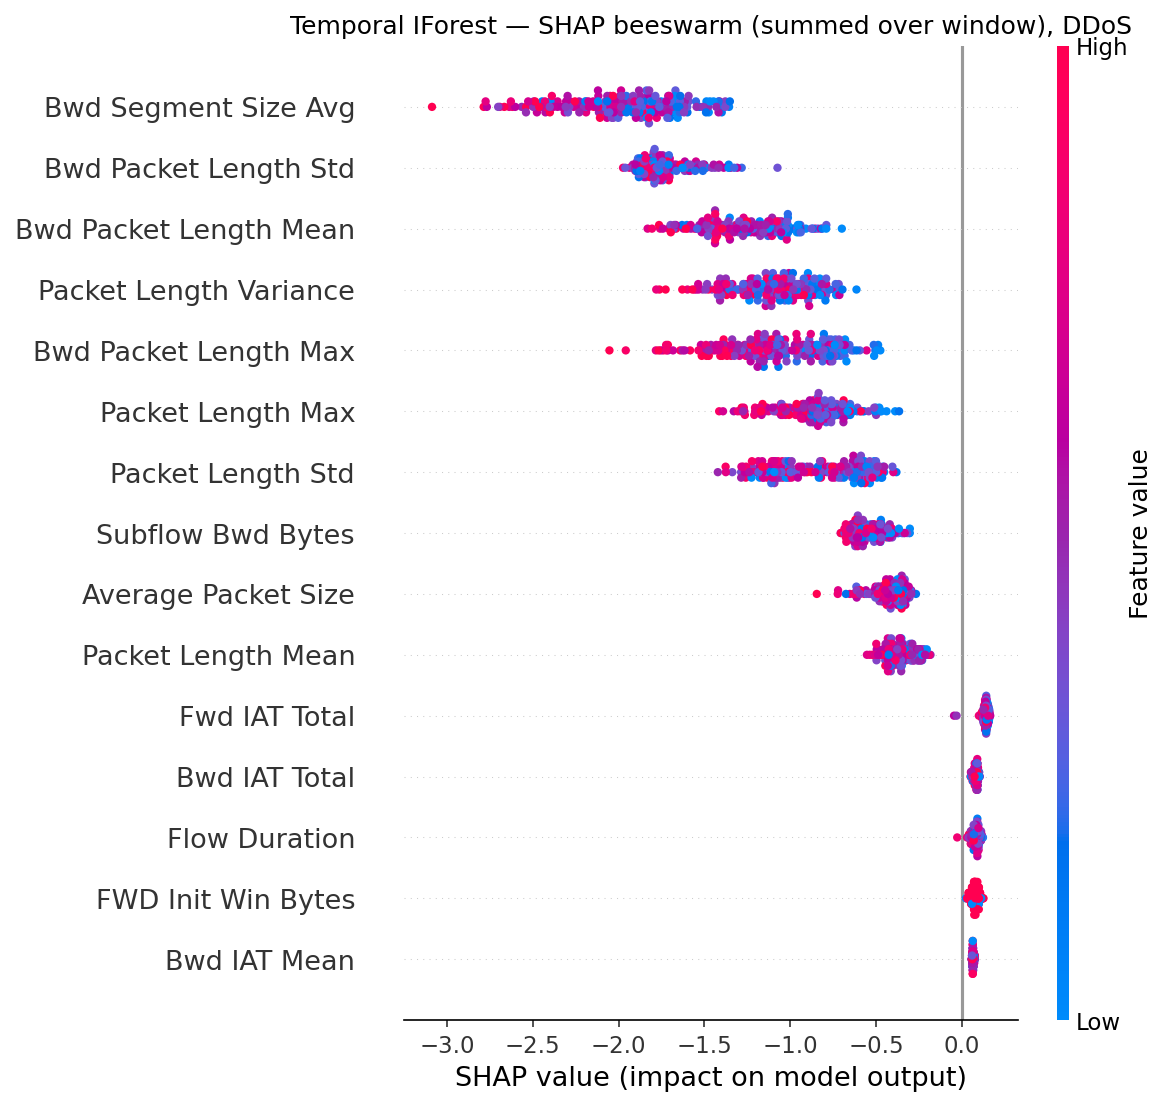
\includegraphics[width=0.48\textwidth,keepaspectratio]{../../data/explainability/cicids_temporal_shap/2/ddos_beeswarm.png}%
\hspace{0.02\textwidth}%
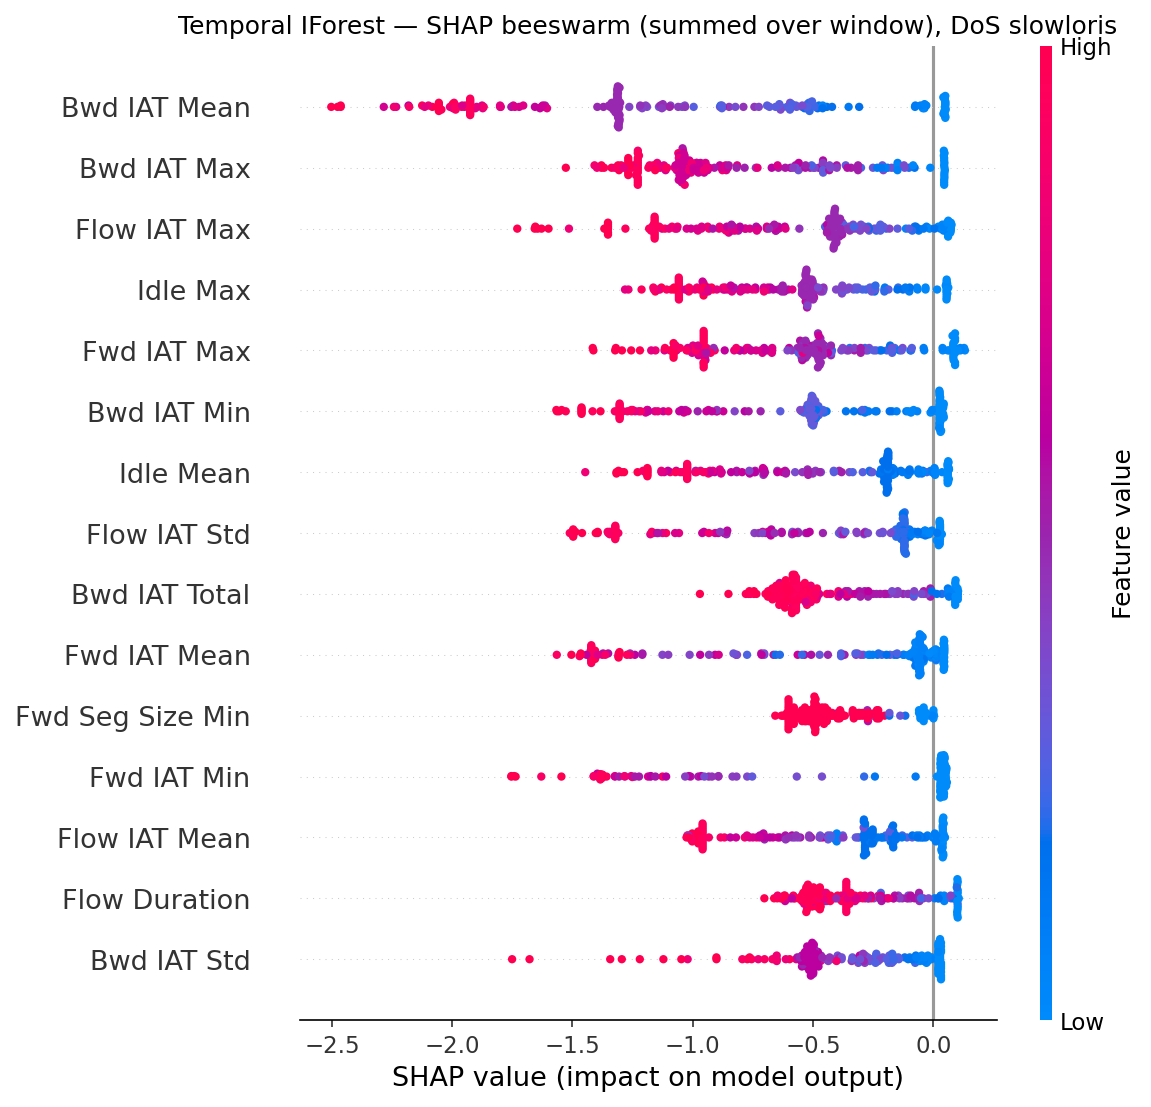
\includegraphics[width=0.48\textwidth,keepaspectratio]{../../data/explainability/cicids_temporal_shap/2/dos_slowloris_beeswarm.png}
\caption{Temporal IForest -- SHAP beeswarm per feature, DDoS windows (left) and DoS slowloris windows (right), collapsing the 16-timestep axis by summing each feature's SHAP contribution across the window and coloring by that feature's mean value across the window. DoS slowloris shows a clean monotonic relationship -- high inter-arrival-time values drive strongly negative (anomalous) SHAP, low values push near zero -- consistent with the slow, connection-holding behaviour the attack is named for. DDoS shows a noisier value-to-sign relationship for its backward-packet-length features, and a wider per-window spread than the mean-only view in Figure~\ref{fig:explain-temporal-shap} suggests on its own.}
\label{fig:explain-temporal-beeswarm}
\end{figure}

The final timestep -- the one paired with AE+Context in the ensemble -- carries only 6--8\% of total attribution mass across all four classes, close to the 6.25\% uniform baseline for a 16-step window, rather than dominating it. The top features also match each attack's known mechanism: DDoS and DoS GoldenEye attribution concentrates on backward-packet-length statistics (\texttt{Bwd Packet Length Std/Mean/Max}, \texttt{Packet Length Variance}), consistent with a volumetric flood; DoS Slowhttptest and DoS slowloris attribution concentrates on inter-arrival-time statistics (\texttt{Fwd/Bwd IAT Std/Max}, \texttt{Idle Mean/Max}), consistent with the slow, connection-holding behaviour these attacks are named for. This confirms the initial assumption: Temporal IForest's advantage on these classes reflects genuinely disjoint temporal evidence, not a relabeled copy of one flow's static features -- supporting the ``disjoint feature regime'' premise behind pairing it with AE+Context.

\subsection{AE+Context: SHAP Dominated by Host-Context Features}

The mirror premise is that AE+Context's advantage on its own strong classes -- DDoS and PortScan, per Chapter~\ref{ch:results} -- traces to the 9 \texttt{ctx\_*} host-context features unique to its feature set, rather than to the same flow-level features Temporal IForest already sees. If instead AE+Context's attribution spreads across ordinary flow features, its complementarity with Temporal IForest would be coincidental rather than a genuinely disjoint evidence source.

SHAP was computed with \texttt{GradientExplainer} on AE+Context's reconstruction error, on 200 samples each of PortScan and DDoS, and the 15 features with the highest mean $|\text{SHAP}|$ were ranked for each class.

\begin{figure}[H]
\centering
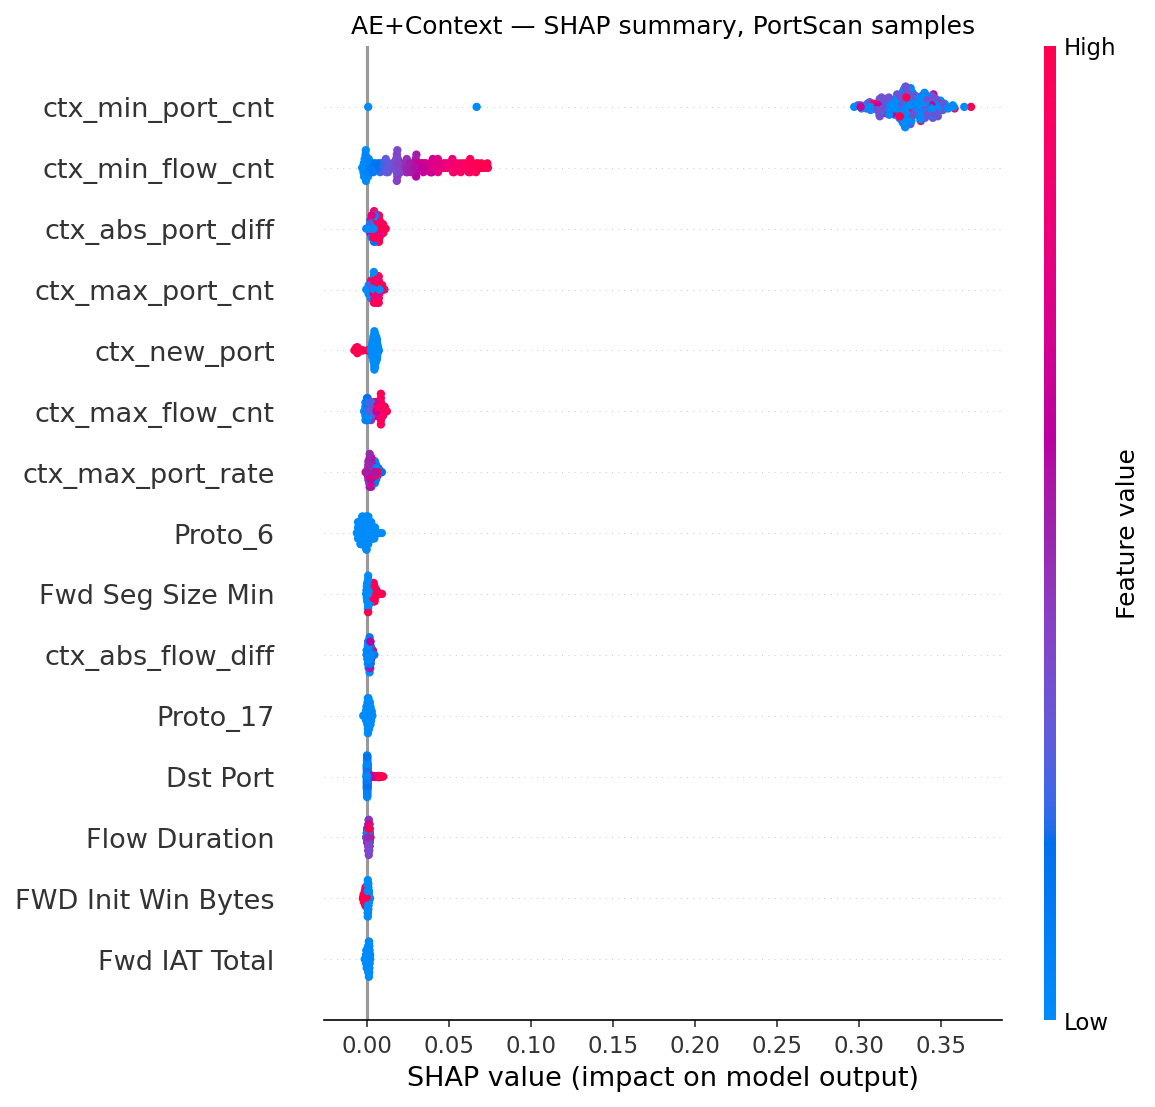
\includegraphics[width=0.75\textwidth]{../../data/explainability/cicids_shap_portscan/5/autoencoder_context_portscan_shap.png}
\caption{AE+Context -- SHAP summary plot, PortScan samples. \texttt{ctx\_min\_port\_cnt} dominates with a tight, uniformly positive-SHAP cluster well separated from every other feature; the remaining top rows are almost entirely \texttt{ctx\_*} host-context features, with ordinary flow features only appearing near the bottom of the ranking.}
\label{fig:explain-ae-context-portscan-shap}
\end{figure}

\begin{center}
\begin{tabular}{@{}lcc@{}}
\toprule
 & \texttt{ctx\_*} features in top 15 & Leading feature (mean $|\text{SHAP}|$) \\
\midrule
PortScan & 8/15 & \texttt{ctx\_min\_port\_cnt} (0.324) \\
DDoS     & 7/15 & \texttt{ctx\_min\_port\_cnt} (0.234) \\
\bottomrule
\end{tabular}
\end{center}

For both classes, \texttt{ctx\_min\_port\_cnt} and \texttt{ctx\_min\_flow\_cnt} dominate by roughly an order of magnitude over every ordinary flow feature: on PortScan, \texttt{ctx\_min\_port\_cnt}'s attribution (0.324) is nearly 70$\times$ the next-highest ordinary feature, \texttt{Fwd Seg Size Min} (0.0023); on DDoS it is over 6$\times$ the leading ordinary feature, \texttt{Bwd Packet Length Std} (0.035). Six of the nine \texttt{ctx\_*} features appear in both classes' top-15 lists, with only \texttt{ctx\_min\_port\_rate} absent from both. This confirms the mirror premise: AE+Context's advantage on these classes is driven almost entirely by host-context evidence unavailable to Temporal IForest, not by the ordinary flow features the two models share.

Taken together with \S\ref{sec:explain-temporal-window}'s result for Temporal IForest, the two halves of the disjoint-feature-regime premise both hold: Temporal IForest's strong classes are explained by evidence spread across the 16-flow window (packet-length statistics for volumetric floods, inter-arrival-time statistics for slow-drip attacks), and AE+Context's strong classes are explained by host-context features that exist only in its own feature set. The proposed ensemble's complementary coverage is therefore backed by genuinely non-overlapping evidence between its two members, not by two rankings that merely happen to differ on which classes they cover.

\subsection{Building the Combined Score}
\label{sec:explain-ensemble-build}

Confirming the disjoint-evidence premise does not by itself establish that combining the two scores works in practice. Realizing the ensemble sketched in Chapter~\ref{ch:results} requires pairing, for every flow $f$ in the test set, AE+Context's own per-flow score $s_{AE}(f)$ with Temporal IForest's score for the 16-flow window \emph{ending} at $f$ -- the same causal, non-leaking choice validated in the previous subsection via last-flow labeling. Since the two preprocessing pipelines reorder flows differently before saving their respective test arrays (AE+Context sorts globally by timestamp; Temporal IForest sorts per source-IP host), the two score arrays are not aligned index-for-index and must be re-aligned by flow identity, recovering each flow's original row position in both pipelines' shared, pre-sort input.

Once aligned, the two raw scores cannot be combined directly: AE+Context's score is a mean-squared reconstruction error with no fixed scale, and Temporal IForest's score is a negated mean path length, and the two live on entirely different numeric ranges. Some normalization is required before either a weighted average or a max can be meaningful. Each model's normalization statistics are computed on that same model's own \emph{benign training} scores only, never on test data, to avoid leaking test-set anomaly information into the fusion.

\subsection{Two Fusion Rules, Two Normalizations}
\label{sec:explain-ensemble-fusion}

Two combination rules were tested. \textbf{Weighted soft voting} takes a convex combination of the two normalized scores, $s_{\text{soft}}(f) = w \cdot \hat{s}_{AE}(f) + (1-w) \cdot \hat{s}_{IF}(f)$, swept over $w \in \{0.3, \dots, 0.7\}$. \textbf{Max-rule fusion} instead takes $s_{\text{max}}(f) = \max(\hat{s}_{AE}(f), \hat{s}_{IF}(f))$ -- an OR-like combiner intended to match the disjoint-evidence story more directly: either model's confidence alone should be enough to flag a flow.

The first normalization attempted, standard $z$-scoring against each model's own benign training mean and standard deviation, turned out to be a dead end rather than a genuine test of either fusion rule. AE+Context's reconstruction-error $z$-scores are extremely heavy-tailed (maximum $z \approx 2366$ on the test set, with the 99.9th percentile of \emph{benign} flows alone already at $z \approx 227$), while Temporal IForest's $z$-scores stay tightly bounded (maximum $z \approx 21$). Under $z$-score normalization, a handful of extreme AE+Context outliers dominate any linear combination or max regardless of the weight assigned to Temporal IForest: max-rule and every soft-vote weight tested reproduced AE+Context's own per-class ranking almost exactly (e.g.\ GoldenEye AP stayed at $0.215$--$0.216$ across all five weights, against AE+Context alone's $0.215$), rather than showing any influence from Temporal IForest's much stronger $0.627$ standalone score on that class. This is a normalization artifact, not evidence that fusion does not help -- it does not actually test the ensemble hypothesis.

Replacing $z$-score with rank normalization -- mapping each test score to its percentile within that model's own benign training-score distribution, via the empirical CDF -- removes this problem by construction: every normalized score is bounded to $[0,1]$ regardless of how extreme the raw value is, so neither model's tail can dominate the other's by sheer magnitude. All results below use rank normalization.

\subsection{Per-Class Coverage vs.\ Aggregate AP}
\label{sec:explain-ensemble-results}

\begin{center}
\begin{tabular}{@{}lccccc@{}}
\toprule
 & DDoS & PortScan & GoldenEye & Slowhttptest & slowloris \\
\midrule
AE+Context alone        & 0.882 & \textbf{0.924} & 0.292 & 0.013 & 0.025 \\
Temporal IForest alone  & \textbf{0.956} & 0.123 & 0.611 & 0.578 & 0.560 \\
Max-rule (rank)         & 0.882 & 0.923 & 0.292 & 0.060 & 0.083 \\
Soft-vote $w=0.4$ (rank) & 0.977 & 0.228 & \textbf{0.801} & \textbf{0.205} & \textbf{0.319} \\
Soft-vote $w=0.7$ (rank) & 0.977 & 0.358 & 0.821 & 0.140 & 0.245 \\
\bottomrule
\end{tabular}
\end{center}

Aggregate AP over the full row-aligned test set actually \emph{favors} the variants that change the least: max-rule (aggregate AP $0.943$) and AE+Context alone ($0.941$) both edge out soft-vote $w=0.4$ ($0.841$), simply because DDoS and PortScan together account for over 250{,}000 of the roughly 434{,}000 positive flows in this evaluation, while GoldenEye, Slowhttptest, and slowloris combined account for barely 13{,}000. An aggregate metric dominated by two classes' raw volume is exactly the wrong lens for judging whether an ensemble motivated by \emph{per-class coverage} actually delivers it, so \S\ref{sec:cic-per-attack}'s per-class breakdown, not the aggregate table, is the right basis for evaluating this ensemble -- consistent with how every other per-attack-type claim in this thesis is judged.

Read per-class, max-rule falls short of its own premise: because it is an OR over two scores, it inherits the \emph{union} of both models' false-positive tendencies rather than only their true positives, so on GoldenEye/Slowhttptest/slowloris it barely moves off AE+Context's own weak scores ($0.292 \to 0.292$, $0.013 \to 0.060$, $0.025 \to 0.083$) despite Temporal IForest's much stronger standalone numbers on exactly these classes. Soft voting shows the opposite failure mode on PortScan: because it averages rather than maxes, and Temporal IForest is actively poor on PortScan ($0.123$, well below AE+Context's $0.924$) rather than merely uninformative, blending pulls PortScan's ranking down substantially ($0.924 \to 0.228$ at $w=0.4$) even while lifting GoldenEye from $0.292$ to $0.801$.

Neither rule is a free win, but soft voting is the more defensible choice for a coverage-motivated ensemble: its \emph{weakest} covered class ($0.205$, Slowhttptest, at $w=0.4$) clears both standalone models' own weakest classes -- AE+Context's $0.013$ (Slowhttptest) and Temporal IForest's $0.123$ (PortScan) -- something neither standalone model nor max-rule fusion achieves. This is a genuine, if partial, realization of the ensemble idea from Chapter~\ref{ch:results}: rank-normalized soft voting measurably widens the floor of attack-class coverage, at the explicit cost of PortScan detection quality, rather than the free lunch the original aggregate-level framing implied. A deployment that must retain AE+Context's near-complete PortScan coverage would instead need a class-aware combination rule (e.g.\ routing PortScan-like flows to AE+Context alone) rather than a single global weight -- left as future work.
